\chapter{Diagonalización}

\section{Motivación: Google Page Rank}

El éxito inicial del motor de búsquedas de Google se debe en gran parte al algoritmo desarrollado para rankear las páginas, es decir, ordenarlas por orden de importancia, y de esa forma poder mostrar a los usuarios resultados relevantes.

¿Cómo determinar si una página es relevante? Una primer medida de relevancia es considerar la cantidad de otras páginas que tienen un enlace a esa página. Sin embargo, con este criterio tan simple, no distinguimos si las páginas que enlazan a cada página son importantes o no. Queremos darle mayor relevancia a enlaces provenientes de páginas relevantes, y caemos en una especie de círculo vicioso.

Podemos resumir la solución propuesta por Google de la siguiente forma.
Consideremos que tenemos 11 páginas, que contienen enlaces entre las distintas página. Una flecha en el gráfico indica que la página de partida tiene un enlace a la página de llegada.

\begin{center}
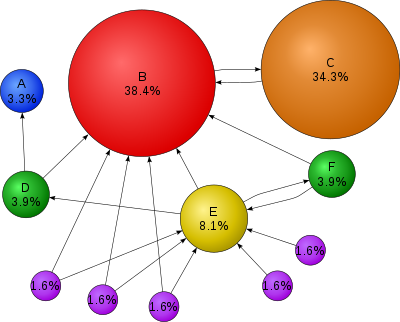
\includegraphics[scale=.5]{400px-PageRanks-Example.png}
\end{center}

Como podemos ver, la página B es relevante porque recibe enlaces desde muchas páginas. La página C en cambio es relevante porque recibe un enlace de B, que es una página relevante. ¿Cómo podemos definir la relevancia?
Pensamos que realizamos el siguiente experimento: ponemos a 1.000.000 de personas a navegar por internet. Inicialmente eligen una página cualquiera al azar y luego cada segundo cambian de página siguiendo algún link al azar de la página en la que están.
Después de varios segundos, ¿cuántos visitantes habrá en cada página?

Podemos modelar esto llamando $\vb^{(0)} \in \R^{11}$ a la cantidad inicial de visitantes en cada sitio, y $\vb^{(k)}$ a la cantidad de visitantes luego de $k$ segundos. Vamos a ver que podemos construir una matriz $\Ab \in \R^{11 \times 11}$, llamada matriz de transición, tal que
$$
\vb^{(k)} = \Ab \vb^{(k-1)}
$$
y recursivamente,
$$
\vb^{(k)} = \Ab^k \vb^{(0)}.
$$

Por lo tanto, para estudiar este proceso, nos interesa poder calcular potencias altas de matrices, o predecir su comportamiento.

Podemos preguntarnos también si existe un límite del proceso, es decir, si luego de varios segundos, la cantidad de visitantes en cada página se mantiene estable. En ese caso, el vector límite debe cumplir la relación
$$
\Ab \vb^{\infty} = \vb^{\infty}.
$$

Los vectores con esta propiedad se llaman autovectores, y es el tema principal de este capítulo.




\section{Autovalores y autovectores}

Dada una matriz cuadrada $\Ab \in \K^{n \times n}$, un vector $\vb \in \K^n$ no nulo tal que
$$
\Ab \vb = \lambda \vb, \text{ para algún } \lambda \in \K
$$ se llama \emph{autovector} de $\Ab$ con \emph{autovalor} $\lambda$.

\textbf{Ejemplo.} Buscamos los autovalores y autovectores de la matriz
$\Ab = \begin{pmatrix} 2 & 3 \\ 2 & 1 \end{pmatrix}$. Tenemos que
encontrar $\vb$ y $\lambda$ tales que $\Ab \vb = \lambda \vb$. El
término de la derecha podemos reescribirlo como $\lambda \Ib \vb$, y esto
nos permite agrupar:
$$(\Ab - \lambda \Ib) \vb = 0,$$
que en nuestro caso queda
$$
\begin{pmatrix}
2 - \lambda & 3 \\
2 & 1 - \lambda
\end{pmatrix}
\begin{pmatrix} v_1 \\ v_2 \end{pmatrix} =
\begin{pmatrix} 0 \\ 0 \end{pmatrix},
$$

Si el determinante de $\Ab - \lambda \Ib$ es no nulo, el sistema tiene
solución única $(v_1, v_2) = (0,0)$. Como estamos buscando vectores no
nulos, debemos encontrar $\lambda$ tal que $\det(\Ab - \lambda \Ib) = 0$.

Calculamos
$$\det(\Ab  - \lambda \Ib) = (2 - \lambda)(1 - \lambda ) - 6 = \lambda^2 - 3 \lambda - 4.$$

Esta ecuación es un polinomio de grado 2 en $\lambda$ y tiene raíces
$$\lambda_1 = -1 \quad \text{y} \quad \lambda_2 = 4.$$
Estos son los autovalores de $\Ab$.

Para calcular los autovectores correspondientes a esos autovalores,
calculamos los núcleos de las matrices $$
\Ab - (-1) \Ib_2 = \begin{pmatrix} 3 & 3 \\ 2 & 2 \end{pmatrix} \quad \text{ y } \quad \Ab - (4) \Ib_2 = \begin{pmatrix} -2 & 3 \\ 2 & -3 \end{pmatrix}.
$$

\begin{Shaded}
\begin{lstlisting}[language=python]
import numpy as np
import scipy.linalg

A = np.array([[2, 3], [2, 1]])
A1 = A - (-1) * np.eye(2)
print(scipy.linalg.null_space(A1))
\end{lstlisting}
\end{Shaded}

\begin{verbatim}
%% [[-0.70710678]
%%  [ 0.70710678]]
\end{verbatim}

\begin{Shaded}
\begin{lstlisting}[language=python]
import numpy as np
import scipy.linalg

A = np.array([[2, 3], [2, 1]])
A1 = A - (-1) * np.eye(2)
print(scipy.linalg.null_space(A1))
\end{lstlisting}
\end{Shaded}

\begin{verbatim}
%% [[0.83205029]
%%  [0.5547002 ]]
\end{verbatim}

El comando \texttt{null\_space} normaliza los vectores a norma-2 igual a 1. Podemos verificar que el espacio de autovectores correspondiente a
$\lambda_1 = -1$ es $$E_{\lambda_1} = \langle (1, -1)\rangle$$ y el
espacio de autovectores correspondiente a $\lambda_2 = 4$ es
$$E_{\lambda_2} = \langle (3, 2)\rangle.$$

Es decir, por ejemplo, $(1, -1)$ es autovector de $\Ab$ de autovalor $-1$,
como también lo es cualquier múltiplo no nulo de ese vector. En este
caso, obtuvimos que el espacio de autovectores de cada autovalor tiene
dimensión 1, o abusando un poco la notación, que a cada autovalor le
corresponde un único autovector.

Repasando,
\begin{itemize}
\item   Los \emph{autovalores} de una matriz $\Ab \in \K^{n \times n}$ ($\K = \R$ o $\C$) son los
    valores $\lambda \in \C$ para los cuales
    $\det(\Ab - \lambda \Ib_n) = 0$.
\item   El espacio de autovalores de un autovalor $\lambda$ es el núcleo de
    la matriz $\Ab - \lambda \Ib_n$.
\item   Si $\lambda$ es autovalor, el núcleo siempre tiene dimensión mayor o
    igual que 1.
\item   Si el núcleo tiene dimensión exactamente 1, decimos informalmente
    que el autovalor $\lambda$ tiene un único autovector.
\end{itemize}

\begin{defi}
Dada $\Ab \in  \Knn$, llamamos \emph{polinomio característico} de $\Ab$ al determinante
$$
\chi_{\Ab}(\lambda) = \det(\Ab - \lambda \Ib).
$$
\end{defi}

Los autovalores de $\Ab$ son las raíces de $\chi_{\Ab}(\lambda)$. El polinomio $\det(\lambda \Ib - \Ab)$ es un polinomio mónico con las mismas raíces que $\det(\lambda \Ib - \Ab)$, y llamamos indistintamente polinomio característico a cualquiera de estos dos polinomios.


\textbf{Ejercicio.} Calcular el polinomio característico, los autovalores y autovectores de la matriz
$$B = \begin{pmatrix} 2 & 0 & 0 \\ 0 & 3 & 4 \\ 0 & 4 & 9 \end{pmatrix}.$$

\textbf{Ejemplo.} Verificamos en \python los cálculos para las dos matrices $\Ab$ y
$\Bb$ utilizando el comando \texttt{linalg.eig} de \texttt{numpy}.

\begin{Shaded}
\begin{lstlisting}[language=python]
A = np.array([[2, 3], [2, 1]])
e = np.linalg.eig(A)   # e es una lista con dos elementos
print("Autovalores: ", e[0])   # El primer elemento es un array
                               # de autovalores
print("Autovectores:\n", e[1]) # El segundo elemento es una matriz
                               # con los autovectores como columnas.
\end{lstlisting}
\end{Shaded}

\begin{verbatim}
%% Autovalores:  [ 4. -1.]
%% Autovectores:
%%  [[ 0.83205029 -0.70710678]
%%  [ 0.5547002   0.70710678]]
\end{verbatim}

\textbf{Ejercicio.} Calcular en \python los autovalores y los autovectores
asociados a cada autovalor para las siguientes matrices.

\begin{enumerate}
\item $\Ab =\begin{pmatrix} -1 & 4 & -2 \\ -3 & 4 & 0 \\ -3 & 1 & 3 \end{pmatrix}$
\item $\Ab = \begin{pmatrix} 0 & 0 & 2 & 1 \\ 1 & 0 & 1 & 0 \\ 0 & 1 & -2 & 0 \\ 0 & 0 & 0 & 1 \end{pmatrix}$
\end{enumerate}

Vamos a utilizar la siguiente propiedad más adelante.

\begin{prop}
Para $\Ab \in \Rnn$, los autovalores de $\Ab$ y $\Ab^T$ son los mismos.
\end{prop}

\begin{proof}
Recordemos que para cualquier $\Ab \in \Rnn$, $\det(\Ab) = \det(\Ab^T)$.

Los autovalores de $\Ab$ son las raíces del polinomio característico $p_{\Ab}(\lambda) = \det(\Ab - \lambda \Ib)$ y los autovalores de $\Ab^T$ son las raíces del polinomio característico $p_{\Ab^T}(\lambda) = \det(\Ab^T - \lambda \Ib)$. Como $(\Ab - \lambda \Ib)^T = \Ab^T - \lambda \Ib$, ambos determinantes son iguales y por lo tanto las raíces son las mismas.
\end{proof}



\section{Diagonalización}

Como vimos, podemos pensar una matriz $\Ab \in \K^{n \times n}$ como una
transformación lineal de $T_{\Ab}: \K^n \rightarrow \K^n$ dada por
$T_{\Ab}(\vb) = \Ab \cdot \vb$ para $\vb \in \K^n$. En este caso estamos pensando
que tanto el vector $\vb$ como $T_{\Ab}(\vb)$ están expresados en coordenadas de
la base canónica. Veamos cómo cambia la matriz de una transformación cuando expresamos los vectores en otra base.

\begin{ejemplo} Continuando el ejemplo anterior, consideramos
$\Ab = \begin{pmatrix} 2 & 3 \\ 2 & 1 \end{pmatrix}$ y la transformación asociada
$$f(\vb) = T_{\Ab}(\vb) = \Ab \vb = \begin{pmatrix} 2 & 3 \\ 2 & 1 \end{pmatrix} \begin{pmatrix} v_1 \\ v_2 \end{pmatrix}.$$

Para esta transformación, vale
$$
\begin{aligned}
T((1,0)) &= (2, 3) \\
T((0,1)) &= (2, 1)
\end{aligned}
$$

También vimos que $\wb_1 = (1,-1)$ y $\wb_2 = (3,2)$ son autovectores de $\Ab$ con autovalores $-1$ y $4$ respectivamente.
Si tomamos la base $\B = \{\wb_1, \wb_2\}$, la transformación en esta base toma una forma más simple:
$$
\begin{aligned}
T(\wb_1) &= -\wb_1 \\
T(\wb_2) &= 4\wb_2
\end{aligned}
$$
o si escribimos a estos vectores en las coordenadas de la base $\B$, obtenemos
$$
\begin{aligned}
T((1,0)_\B) &= (-1,0)_\B \\
T((0,1)_\B) &= (0,4)_\B \\
\end{aligned}
$$

Podemos entonces considerar la matriz de la transformación $T$ expresada en coordenadas de la base $\B$ y llamamos $[f]_\B$ a esta matriz. Obtuvimos:
$$
[f]_\B = \begin{pmatrix} -1 & 0 \\ 0 & 4 \end{pmatrix}.
$$

\end{ejemplo}

En general, tenemos el siguiente resultado.

\begin{prop}
Sea $\Ab \in \Knn$ tal que existe una base $\B = \{\wb_1, \dots, \wb_n\}$ de $\Kn$ formada por autovectores de $\Ab$, con autovalores $\lambda_1, \dots, \lambda_n \in \C$ (no necesariamente distintos). Sea $f: \Kn \rightarrow \Kn$ la transformación asociada, $f(\vb) = \Ab \vb$. La matriz de la $f$ en la base $\B$ es diagonal,
$$
[f]_\B =
\begin{pmatrix} \lambda_1 & & 0 \\ & \ddots & \\ 0 & & \lambda_n \end{pmatrix}
$$

\end{prop}

Estudiamos ahora la relación entre la matriz original $\Ab$ y la matriz $[f]_\B$ en la base de autovectores.

Recordemos que dada una base $\B = \{\wb_1, \dots, \wb_n\}$ de $\Kn$ y un vector $\vb \in \Kn$ con coordenadas en la base $\B$
$$
\vb = (u_1, \dots, u_n)_\B,
$$
podemos encontrar las coordenadas de $\vb$ en la base canónica mediante la multiplicación
$$
\vb_\E = \Cb_{\B\E} \vb_B,
$$
donde $\Cb_{\B\E}$ es la matriz de cambio de base de $\B$ a $\E$,
$$\Cb_{\B\E} = \begin{pmatrix} \mid & \mid & & \mid \\ {\bb}_{1} & {\bb}_{2} & \cdots & {\bb}_{n}\\ \mid & \mid & & \mid \\ \end{pmatrix}.$$

Si en cambio, dadas las coordenadas canónicas de un vector $\vb = (v_1, \dots, v_n)_\E$, queremos encontrar las coordenadas en la base $\B$, realizamos la multiplicación
$$
\vb_\B = \Cb_{\E\B} \vb_E,
$$
donde $\Cb_{\E\B}$ es la matriz de cambio de base de $\E$ a $\B$, que podemos calcular invirtiendo la matriz $\Cb_{\B\E}$,
$$
\Cb_{\E\B} = \Cb_{\B\E}^{-1}.
$$

Por lo tanto, si $f$ es una transformación lineal dada en coordenadas de la base canónica por una matriz $\Ab$, podemos obtener la matriz de la transformación en una base $\B$ (es decir que
tanto $\vb$ como $T_{\Ab}(\vb)$ estén expresados en coordenadas de la base $\B$)
aplicando el siguiente cambio de base a la matriz $\Ab$:
$$
\Ab_\B = \Cb_{\E\B} \Ab \Cb_{\B\E}.
$$

Vemos que tanto $\Ab$ como $\Ab_\B$ representan la misma transformación
lineal pero expresada en distintas bases. En este caso, decimos que las
matrices son \emph{semejantes}.

Más generalmente, dos matrices $\Ab, \Bb$ son \emph{semejantes} si existe una
matriz inversible $\Cb$ tal que
$$\Bb = \Cb^{-1} \Ab \Cb.$$

\textbf{Ejemplo.} Continuamos el ejemplo
$\Ab = \begin{pmatrix} 2 & 3 \\ 2 & 1 \end{pmatrix}$. Vimos que $\Ab$ tiene
autovalores $\lambda_1 = -1$ y $\lambda_2 = 4$ con autovectores
$v_{1} = (1, -1)$ y $v_{2} = (3, 2)$ respectivamente. Estos autovectores
forman una base de $\R^2$. Si expresamos la matriz $\Ab$ en la base
$\Bb = \{v_{1}, v_2\}$ obtenemos
$$
\Ab_\B = \begin{pmatrix} -1 & 0 \\ 0 & 4 \end{pmatrix}
$$
(en las columnas de $\Ab_\B$ ponemos las imágenes de los vectores de la
base $\B$ expresados también en coordenadas de la base $\B$).

Verificamos en \python.

\begin{Shaded}
\begin{lstlisting}[language=python]
A = np.array([[2, 3], [2, 1]])
e = np.linalg.eig(A)
C_BE = e[1]
C_EB = np.linalg.inv(C_BE)
print("A_B = \n", C_EB @ A @ C_BE)
\end{lstlisting}
\end{Shaded}

\begin{verbatim}
%% A_B =
%%  [[ 4.00000000e+00  0.00000000e+00]
%%  [-5.55111512e-17 -1.00000000e+00]]
\end{verbatim}

La siguiente propiedad resume lo que acabamos de ver.

\begin{prop}
Si $\Ab \in \K^{n \times n}$ y $\B = \{\bb_1, \dots, \bb_n\}$
es una base de $\K^n$ formada por autovectores de $\Ab$ con autovalores
$\{\lambda_1, \dots, \lambda_n\}$, entonces tomando

\begin{itemize}
\item   $\Db$ la matriz diagonal de autovalores,
    $\Db = \begin{pmatrix} \lambda_1 & & \\ & \ddots & \\ & & \lambda_n \end{pmatrix}$,
\item   $\Cb$ la matriz de autovectores de $\Ab$,
    $\Cb = \begin{pmatrix} \vert & & \vert \\ \bb_1 & \dots & \bb_n \\ \vert & & \vert \end{pmatrix}$
obtenemos la diagonalización de la matriz $\Ab$
$$
\Ab = \Cb \Db \Cb^{-1} \quad \text{y} \quad \Db = \Cb^{-1} \Ab \Cb.
$$
\end{itemize}
\end{prop}

\textbf{Ejercicio.} Calcular en Python los autovalores y autovectores de las
siguientes matrices. Según los resultados obtenidos, ¿alguna de estas
matrices es diagonalizable?

\begin{enumerate}
\item  $\Ab = \begin{pmatrix} 1 & 1 & 0 \\ 0 & 1 & 1 \\ 0 & 0 & 1 \end{pmatrix}$
\item  $\Ab = \begin{pmatrix} -1 & 3 & -1 \\ -3 & 5 & -1 \\ -3 & 3 & 1 \end{pmatrix}$
\end{enumerate}

Para la matriz que resulte diagonalizable, ¿cuál es la base $\B$ de
autovectores? ¿Quién es $\Db$? Hallar $\Cb$ tal que $\Ab = \Cb \Db \Cb^{-1}$ .

%\begin{lstlisting}[language=R]
%A = matrix(c(1, 1, 0, 0, 1, 1, 0, 0, 1), nrow = 3, byrow = TRUE)
%e = eigen(A)
%print(e)
%
%R(e$vectors)
%print(round(e$vectors, 4))
%\end{lstlisting}
%
%\begin{lstlisting}[language=R]
%A = matrix(c(-1, 3, -1, -3, 5, -1, -3, 3, 1), nrow = 3, byrow = TRUE)
%e = eigen(A)
%print(e)
%
%# Verificamos que tenemos el rango correcto
%R(e$vectors)
%
%#Construimos la matriz diagonal
%D = diag(e$values)
%print(D)
%
%#Construimos las matrices de cambio de base
%
%C = e$vectors
%print(round(C, 4))
%
%C_inv = solve(C)
%
%# Verificamos
%print(C_inv %*% A %*% C)
%print(round(C_inv %*% A %*% C, 4))
%
%print(round(C %*% D %*% C_inv),4)
%
%\end{lstlisting}[language=R]

Como vimos en el ejercicio, no cualquier matriz es diagonalizable.

Dada una matriz $\Ab$, sean $\lambda_1, \dots, \lambda_k$ los autovalores
distintos de $\Ab$. Definimos $E_{\lambda_i}$ el espacio de autovectores
asociados al autovalor $\lambda_i$. $\Ab$ es diagonalizable si
$$
\dim(E_{\lambda_1}) + \dim(E_{\lambda_2}) + \dots +\dim(E_{\lambda_k}) = n.
$$
En particular, como $\dim(E_\lambda) \ge 1$ para $\lambda$ autovector
(¿por qué?), si $\Ab$ tiene $n$ autovalores distintos, $\Ab$ es
diagonalizable.

\begin{ejercicio}
Para cada una de las siguientes matrices, calcular en \python los
autovalores, las dimensiones de los espacios asociados a cada autovalor
y determinar si las matrices son diagonalizables.

\begin{enumerate}
\item   $\Ab = \begin{pmatrix} 101 & 2 & 3 & 4 \\ 1 & 102 & 3 & 4 \\ 1 & 2 & 103 & 4 \\ 1 & 2 & 3 & 104 \end{pmatrix}$
\item   $\Ab = \begin{pmatrix} 5 & 4 & 2 & 1 \\ 0 & 1 & -1 -1 \\ -1 &-1 &3 & 0 \\ 1 & 1 & -1 & 2 \end{pmatrix}$
\end{enumerate}

%\begin{lstlisting}[language=R]
%A = matrix(c(101,2,3,4,1,102,3,4,1,2,103,4,1,2,3,104), nrow=4)
%#A = matrix(c(5,4,2,1,0,1,-1,-1,-1,-1,3,0,1,1,-1,2), nrow=4)
%\end{lstlisting}

\end{ejercicio}

\subsection{Multiplicidad algebraica y geométrica}
Dada una matriz $\Ab \in \Knn$ y un autovalor $\lambda$ de $\Ab$, definimos:
\begin{itemize}
\item La \emph{multiplicidad aritmética} de $\lambda$ es la multiplicidad de $\lambda$ como raíz del polinomio característico $\chi_{\Ab}$.
\item La \emph{multiplicidad geométrica} de $\lambda$ es la dimensión del espacio de autovectores asociado a $\lambda$, o equivalentemente, la dimensión de $\Nu(\Ab - \lambda \Ib)$.
\end{itemize}

\begin{prop}
Dada una matriz $\Ab \in  \Knn$ y un autovalor $\lambda$ de $\Ab$, la multiplicidad geométrica es siempre menor o igual que la multiplicidad aritmética.
\end{prop}

\begin{proof} Sea $s$ la multiplicidad geométrica de $\lambda$ y $\{\vb_1, \dots, \vb_s\}$ una base de autovectores de $E_{\lambda}$, el espacio de autovectores asociados a $\lambda$. Completamos la base de $E_{\lambda}$ a una base de $\Kn$:
$$
\B = \{\vb_1, \dots, \vb_s, \wb_1, \dots, \wb_{n-s}\}.
$$

Consideramos la matriz de la transformación $f$ definida por $\Ab$ en la base $\B$:
$$
\sbox0{$\begin{matrix}\lambda & & \\ & \ddots & \\ & & \lambda\end{matrix}$}
[f]_\B =\left(
\begin{array}{c|c}
\usebox{0}&\makebox[\wd0]{\large $B$}\\
\hline
  \vphantom{\usebox{0}}\makebox[\wd0]{\large $0$}&\makebox[\wd0]{\large $D$}
\end{array}
\right),
$$
donde el primer bloque es una matriz de $s \times s$.

Utilizando la fórmula para el cálculo de determinantes desarrollando una columna, es fácil ver que
$$
\chi_{[f]_\B}(x) = \det(x\Ib_n - [f]_\B) = (x-\lambda)^s \det (x\Ib_n - [f]_\B).$$

 Ya vimos que $[f]_\B$ y $[f]_\E$ tienen el mismo polinomio característico. Por lo tanto, la multiplicidad algebraica de $\lambda$ como autovalor de $\Ab$ es al menos $s$, como queríamos ver.
\end{proof}

Para una matriz $\Ab \in \Knn$, el polinomio característico tiene grado $n$ y por lo tanto $n$ raíces contando sus multiplicidades. Es decir, que la suma de las multiplicidades aritméticas de todos los autovalores es siempre exactamente $n$. Más aún, autovectores correspondientes a autovalores distintos son linealmente independientes.

\begin{prop}
Dada $\Ab \in \Knn$, sean $\vb_1, \dots, \vb_s$ autovectores de $\Ab$ correspondientes a autovalores distintos $\lambda_1, \dots, \lambda_s$.
El conjunto $\{\vb_1, \dots, \vb_s\}$ es linealmente independiente.
\end{prop}

\begin{proof}
Consideramos una relación de dependencia lineal:
$$
a_1 \vb_1 + a_2 \vb_2 + \dots + a_s \vb_s = 0
$$
y supongamos que es la relación que involucra la menor cantidad posible de vectores, en particular todos los $a_i$ son no nulos.

Si multiplicamos la igualdad por $(\Ab - \lambda_1 \Ib_n)$ obtenemos:
$$
a_1  (\Ab - \lambda_1 \Ib_n) \vb_1 + a_2 (\Ab - \lambda_1 \Ib_n) \vb_2 + \dots + a_s(\Ab - \lambda_1 \Ib_n)  \vb_s = 0,$$
y simplificando,
$$
0 + a_2 (\lambda_2 - \lambda_1)  \vb_2 \dots + a_s(\lambda_s - \lambda_1)  \vb_s = 0,
$$
que es una relación con menos términos no nulos que la anterior, lo cual es un absurdo.
\end{proof}

Combinando este resultado con la propiedad anterior, obtenemos el siguiente resultado.

\begin{prop}
Una matriz $\Ab$ es diagonalizable si para todo autovalor $\lambda$ de $\Ab$, la multiplicidad artimética y la multiplicidad geométrica coinciden.
\end{prop}

\

\subsection{Propiedades de las matrices diagonalizables}

\begin{prop} Si $\Ab = \Cb^{-1} \Db \Cb$,
\begin{itemize}
\item   $\Ab^2 = \Cb^{-1} \Db \Cb \Cb^{-1} \Db \Cb = \Cb^{-1} \Db \Db \Cb = \Cb^{-1} \Db^2 \Cb$
\item   Inductivamente, $\Ab^k = \Cb^{-1} \Db \Cb \dots \Cb^{-1} \Db \Cb = \Cb^{-1} \Db^k \Cb$
\item   Si $\Ab$ inversible, $\Ab^{-1} = (\Cb^{-1} \Db \Cb)^{-1} = \Cb^{-1} \Db^{-1} \Cb$.
\item   Si $p(x) \in \R[x]$, $p(\Ab) = \Cb^{-1} p(\Db) \Cb$.
\end{itemize}
\end{prop}

En todos estos casos, como vimos anteriormente, la función aplicada a
una matriz diagonal se puede calcular fácilmente aplicando la función a
cada elemento de la diagonal.


\subsection{Aplicación}

Consideramos el siguiente problema como ejemplo de aplicación.

Para guardar cadenas de caracteres en la computadora se pueden utilizar distintas codificaciones. Una codificación consiste en asignarla a cada carácter un número y ese número se guarda en binario en la memoria de la computadora. Dependiendo la codificación utilizada pueden utilizarse entre 1 y 4 bytes por carácter.
Supongamos ahora que recibimos un mensaje en el que se han mezclado caracteres guardados utilizando 1 byte y caracteres utilizando 2 bytes, y no sabemos cuáles caracteres usan 1 byte y cuáles usan 2 bytes. ¿De cuántas formas distintas se puede interpretar el mensaje?

Planteando el problema en forma más abstracta, tenemos un tablero de $n \times 1$, y queremos dividir el tablero en bloques, que pueden ser de $1 \times 1$ o de $2 \times 1$. ¿De cuántas formas podemos hacerlo?

Llamamos $a_n$ a esta cantidad. Es posible demostrar la siguiente fórmula recursiva para los valores de la sucesión:
$$
\begin{aligned}
a_1 &= 1 \\
a_2 &= 2 \\
a_{n} &= a_{n-1} + a_{n-2}
\end{aligned}
$$

Es decir, los valores $a_n$ forman una sucesión de Fibonacci. Para utilizar la teoría de transformacion lineales, nos gustaría encontrar una relación lineal entre cada término y el siguiente. Sin embargo, como está planteada la sucesión, cada término depende de los dos anteriores. Aplicamos un truco simple para plantear la relación de forma que cada término dependa solo del anterior. Plantear la ecuación de recurrencia en forma matricial de la siguiente forma:
$$
\begin{pmatrix} a_{n} \\ a_{n-1} \end{pmatrix} =
\begin{pmatrix} 1 & 1 \\ 1 & 0 \end{pmatrix} \begin{pmatrix} a_{n-1} \\ a_{n-2} \end{pmatrix}.
$$

Si llamamos $\Ab = \begin{pmatrix} 1 & 1 \\ 1 & 0 \end{pmatrix}$, obtenemos
$$
\begin{pmatrix} a_{n} \\ a_{n-1} \end{pmatrix} =
\Ab \begin{pmatrix} a_{n-1} \\ a_{n-2} \end{pmatrix} = \Ab \Ab \begin{pmatrix} a_{n-2} \\ a_{n-3} \end{pmatrix} = \dots = (\Ab)^{n-2} \begin{pmatrix} a_{2} \\ a_{1} \end{pmatrix}
$$

Por lo tanto, podemos dar una fórmula cerrada para la sucesión si encontramos una expresión cerrada para la matriz $(\Ab)^{n-2}$. Esto podemos hacerlo diagonalizando la matriz.

Calculamos autovalores y autovectores de $\Ab$ en \python.

\begin{Shaded}
\begin{lstlisting}[language=python]
A = np.array([[1, 1], [1, 0]])
e = np.linalg.eig(A)
print("Autovalores: ", e[0])
print("Autovectores: \n", e[1])
\end{lstlisting}
\end{Shaded}

\begin{verbatim}
%% Autovalores:  [ 1.61803399 -0.61803399]
%% Autovectores:
%%  [[ 0.85065081 -0.52573111]
%%  [ 0.52573111  0.85065081]]
\end{verbatim}

Como hay dos autovalores distintos, podemos diagonalizar $\Ab$. Obtenemos
$$
\Ab = \Cb_{\B\E} \begin{pmatrix} 1.618 & 0 \\ 0 & -0.618 \end{pmatrix} \Cb_{\E\B},
$$
con $\Cb_{\B\E} = \begin{pmatrix} 0.85 & -0.52 \\ 0.52 & 0.85 \end{pmatrix}$ y $\Cb_{\E\B} = \Cb_{\B\E}^{-1}$.

Esto nos permite dar la siguiente expresión para los términos de la sucesión:
$$
\begin{pmatrix} a_{n} \\ a_{n-1} \end{pmatrix} =
\Cb_{\B\E} \begin{pmatrix} (1.618)^{n-2} & 0 \\ 0 & (-0.618)^{n-2} \end{pmatrix} \Cb_{\E\B} \begin{pmatrix} a_{2} \\ a_{1} \end{pmatrix}.
$$

Vemos en particular que los términos de la sucesión crecen con velocidad exponencial. Haciendo las cuentas en forma simbólica, podemos dar una expresión exacta para los términos de la sucesión (los autovalores de la matriz son $\frac{1+\sqrt{5}}{2} y \frac{1-\sqrt{5}}{2}$.










\section{Descomposición de Schur}
Si bien vimos que no toda matriz es diagonalizable, es decir, semejante a una matriz diagonal, vamos a ver que toda la matriz es semejante a una matriz triangular superior con los autovalores en la diagonal. Más aun, la matriz de cambio de base se puede tomar unitaria. En este caso, decimos que las matrices son unitariamente equivalentes. Concretamente, tenemos el siguiente resultado.

\begin{teo}
Dada una matriz $\Ab \in \Knn$ con autovalores $\lambda_1, \dots, \lambda_n$ (no necesariamente distintos), existen matrices $\Ub$ unitaria y $\Tb$ triangular superior tales que
$$
\Ab = \Ub \Tb \Ub^*
$$
y $t_{ii} = \lambda_i$. Es decir, $\Ab$ es unitariamente equivalente a una matriz $\Tb$ triangular superior con los autovalores de $\Ab$ en la diagonal en cualquier orden arbitrario. Si $\Ab \in \Rnn$ y los autovalores de $\Ab$ son reales, la matriz $\Ub$ se puede tomar real y ortogonal.
\end{teo}

Recordemos que para una matriz $\Ub$ unitaria, vale $\Ub^{-1} = \Ub^*$, por lo tanto las matrices $\Ab$ y $\Tb$ son semejantes.

\begin{proof}
Construimos $\Ub$ y $\Tb$ paso a paso.

Tomamos $\lambda_1$ autovalor de $\Ab$ y $\wb_1$ autovector de $\Ab$ con autovalor $\lambda_1$ y $\|\wb_1\|_2 = 1$.

Completando $\{\wb_1\}$ a una base de $\Kn$ y aplicando ortonormalización de Gram-Schmidt, podemos obtener una base ortonormal de $\C^n$,
$$
\{\wb^{(1)}, \zb^{(2)}, \dots, \zb^{(n)}\}.
$$

Construimos la matriz $\Ub_1$ tomando estos vectores como columnas de la matriz. Como la primera columna de $\Ab \Ub_1$ es $\lambda_1 \wb^{(1)}$, obtenemos
$$
\Ub_1^* \Ab \Ub_1 = \left[
\begin{array}{c|c}
\lambda_1 & * \\ \hline
0 & \Ab_1
\end{array}
\right],
$$

Como $\Ub_1^* \Ab \Ub$ y $\Ab$ son semejantes, tienen el mismo polinomio característico. Luego $\Ab_1 \in \C^{(n-1) \times (n-1)}$ tiene autovalores $\lambda_2, \dots, \lambda_n$. Tomamos ahora $\wb^{(2)} \in \C^{n-1}$ autovector normalizado de $\Ab_1$ correspondiente al autovalor $\lambda_2$ y repetimos el procedimiento. Construimos $\Ub_2 \in \C^{(n-1) \times (n-1)}$ unitaria tal que
$$
\Ub_2^* \Ab_1 \Ub_2 = \left[
\begin{array}{c|c}
\lambda_2 & * \\ \hline
0 & \Ab_2
\end{array}
\right],
$$
y definimos
$$
\Vb_2 = \left(
\begin{array}{c|c}
1 & 0 \\ \hline
0 & \Ub_2
\end{array}
\right).
$$

Las matrices $\Vb_2$ y $\Ub_1 \Vb_2$ son unitarias, y $\Vb_2^* \Ub_1^* \Ab \Ub_1 \Vb_2$ tiene la forma
$$
\sbox0{$\begin{matrix}\lambda_1 & * \\ 0 & \lambda_2 \end{matrix}$}
\Vb_2^* \Ub_1^* \Ab \Ub_1 \Vb_2 =\left(
\begin{array}{c|c}
\usebox{0}& \makebox[\wd0]{\large $*$}\\
\hline
    \vphantom{\usebox{0}}\makebox[\wd0]{\large $0$}&\makebox[\wd0]{\large $\Ab_2$}
\end{array}
\right).
$$

Repitiendo este procedimiento, obtenemos matrices unitarias $\Ub_i \in \C^{(n-i+1) \times (n-i+1)}$, $i = 1, \dots, n-1$, y matrices unitarias $\Vb_i \in \Cnn$, $i = 2, \dots, n-1$. La matriz
$$
\Ub = \Ub_1 \Vb_2 \Vb_3 \dots \Vb_{n-1}
$$
es unitaria y $\Ub^* \Ab \Ub$ es la factorización que buscamos.

Si todos los autovalores de $\Ab$ son reales, los autovectores pueden elegirse también reales y todas las operaciones se pueden hacer sobre los reales, lo que prueba la última información.
\end{proof}

\section{Autovalores y autovectores de matrices simétricas y hermitianas}

\textbf{Matrices ortogonales.} Si $\Ab \in \K^{n \times n}$ es unitaria,
    todos sus autovalores cumplen $|\lambda| = 1$.

\textbf{Matrices normales.}
Decimos que una matriz $\Ab$ es normal si conmuta con la matriz adjunta, es decir, si $\Ab \Ab^* = \Ab^* \Ab$.

Recordemos que dos matrices $\Ab$ y $\Bb$ son unitariamente equivalentes si existe $\Ub$ unitaria tal que
$$
\Ub^* \Ab \Ub = \Bb.
$$

\begin{prop}
Si $\Ab$ es normal y $\Bb$ es unitariamente equivalente a $\Ab$, entonces $\Bb$ es normal.
\end{prop}
\begin{proof}
Tenemos que existe $\Ub$ unitaria tal que $\Ub^* \Ab \Ub = \Bb$. Por lo tanto,
$$
\Bb \Bb^* = \Ub^* \Ab \Ub \Ub^* \Ab^* \Ub = \Ub^* \Ab \Ab^* \Ub = \Ub^* \Ab^* \Ab \Ub = \Ub^* \Ab^* \Ub \Ub^* \Ab \Ub = \Bb^* \Bb.
$$
\end{proof}

Decimos que una matriz $\Ab$ es \emph{unitariamente diagonalizable} si existe una matriz $\Ub$ unitaria tal que $\Ub \Ab \Ub^*$ es diagonal. Esto es equivalente a decir que $\Ab$ tiene una base ortonormal de autovectores.

\begin{prop}
Si $\Ab$ es normal, entonces $\Ab$ es unitariamente diagonalizable. En particular, autovectores de $\Ab$ correspondientes a autovalores distintos son ortogonales.
\end{prop}

\begin{proof}
Por la descomposición de Shur, sabemos que existe $\Tb$ triangular superior unitariamente equivalente a $\Ab$.
Por lo tanto, podemos probar el resultado para $\Tb$.

Hacemos la demostración probando mediante cálculos explícitos que una matriz $\Tb$ triangular y normal debe ser diagonal. Tenemos
$$
\begin{pmatrix}
\bar t_{11} & 0           & \cdots & 0 \\
\bar t_{21} & \bar t_{22} & \cdots & 0\\
\vdots      & \vdots      & \ddots & \vdots \\
\bar t_{n1} & \bar t_{n2} & \cdots & \bar t_{nn}\\
\end{pmatrix}
\begin{pmatrix}
t_{11} & t_{12} & \cdots & t_{1n} \\
0      & t_{22} & \cdots & t_{2n} \\
\vdots & \vdots & \ddots & \vdots \\
0      & 0      & \cdots & t_{nn}\\
\end{pmatrix} =
\begin{pmatrix}
t_{11} & t_{12} & \cdots & t_{1n} \\
0      & t_{22} & \cdots & t_{2n} \\
\vdots & \vdots & \ddots & \vdots \\
0      & 0      & \cdots & t_{nn}\\
\end{pmatrix} \begin{pmatrix}
\bar t_{11} & 0           & \cdots & 0 \\
\bar t_{21} & \bar t_{22} & \cdots & 0\\
\vdots      & \vdots      & \ddots & \vdots \\
\bar t_{n1} & \bar t_{n2} & \cdots & \bar t_{nn}\\
\end{pmatrix}.
$$

Comparando la casilla $(1,1)$ del producto a ambos lados,
$$
\bar t_{11} t_{11} = t_{11} \bar t_{11} + \sum_{j = 2}^n t_{1j} \bar t_{j1}.
$$
Recordando que para cualquier $a \in \C$, $a \bar a = \bar a a = |a|^2$, obtenemos
$$
|t_{11}|^2 = |t_{11}|^2  + \sum_{j = 2}^n |t_{1j}|^2.
$$
y por lo tanto
$$
0 = \sum_{j = 2}^n |t_{1j}|^2.
$$
Una suma de términos no-negativos solo puede dar 0 si todos sus términos son 0, luego
$$
t_{1j} = 0, j = 2, \dots, n.
$$

Ahora usamos que la casillas $(2,2)$ de $\Tb^* \Tb$ y $\Tb \Tb^*$ son iguales y obtenemos
$$
\bar t_{22} t_{22} = t_{22} \bar t_{22} + \sum_{j = 3}^n t_{2j} \bar t_{j2},
$$
de donde concluimos
$$
t_{2j} = 0, j = 3, \dots, n.
$$

Repitiendo este mismo argumento para todas las casillas de la diagonal, obtenemos
$$
t_{ij} = 0, \text{ para todo } j > i
$$
y como
$$
t_{ij} = 0, \text{ para todo } j < i
$$
porque $\Tb$ es triangular superior, concluimos que $\Tb$ es diagonal.
\end{proof}




\textbf{Matrices simétricas y hermitianas.} Una matriz $\Ab \in \Rnn$ es simétrica si $\Ab = \Ab^T$. Más generalmente, $\Ab \in \Cnn$ es Hermitiana si $\Ab = \Ab^*$.

\begin{prop}
Si $\Ab$ es Hermitiana, entonces
\begin{enumerate}
\item \label{item:real} $\xb^* \Ab \xb$ es real para todo $\xb \in \Cn$,
\item \label{item:realav} todos los autovalores de $\Ab$ son reales,
\item $\Sb^* \Ab \Sb$ es Hermitiana para toda $\Sb \in \Cnn$.
\end{enumerate}
\end{prop}

\begin{proof}
Para \ref{item:real}, calculamos
$$
\overline{\xb^* \Ab \xb} = (\xb^* \Ab \xb)^* = \xb^* \Ab^* \xb = \xb^* \Ab \xb.
$$
Como el conjugado de $\xb^* \Ab \xb$ es igual a si mismo, es un n\'umero real.

Para \ref{item:realav}, si $\Ab \xb = \lambda \xb$ y suponemos $\xb$ normalizado $\|\xb\|_2 = \xb^* \xb = 1$, entonces
$$\lambda = \lambda \xb^* \xb = \xb^* \lambda  \xb =  \xb^* \Ab  \xb,$$
que es un n\'umero real por \ref{item:real}.

Por \'ultimo, $(\Sb^* \Ab \Sb)^* = \Sb^* \Ab^* \Sb = \Sb^* \Ab \Sb$, y por lo tanto $\Sb^* \Ab \Sb$ es Hermitiana.
\end{proof}

\begin{ejemplo}
Buscamos una base ortogonal de autovectores de
$$
\Ab = \begin{pmatrix} -4 & 2 & -2 \\ 2 & -7 & 4 \\ -2 & 4 & -7 \end{pmatrix}.$$

Calculamos $\det(\Ab - \lambda \Ib_3) = -(\lambda^3 + 18 \lambda^2 + 81 \lambda + 108) = -(\lambda + 12)(\lambda + 3)^2$, por lo tanto hay dos autovalores $\lambda_1 = -12$ y $\lambda_2 = -3$.

Calculando los núcleos de $\Ab - \lambda_i \Ib_3$, $i = 1, 2$, obtenemos los espacios de autovectores
$$
\begin{aligned}
E_{\lambda_1} &= \langle (1, -2, 2) \rangle \\
E_{\lambda_2} &= \langle (2, 1, 0), (2, 0, -1) \rangle
\end{aligned}
$$

Por la Proposición \ref{prop:normal}, los espacios de autovalores correspondientes a distintos autovectores son ortogonales. Por lo tanto, para obtener una base de autovectores ortogonales, solo debemos ortogonalizar cada uno de los autoespacios por separado.

El autovector $(1, -2, 2)$ lo normalizamos a $\frac{\sqrt{5}}{5}(1, -2, 2)$ y para encontrar una base ortonormal de $E_{\lambda_2}$ aplicamos Gram-Schmidt y obtenemos $E_{\lambda_2} = \left\langle \frac{\sqrt{3}}{3}(2, 1, 0), \frac{\sqrt{5}}{15}(2, -4, -5) \right\rangle$.

La base ortogonal de autovectores es $\B = \left\{\frac{\sqrt{5}}{5}(1, -2, 2), \frac{\sqrt{3}}{3}(2, 1, 0), \frac{\sqrt{5}}{15}(2, -4, -5)\right\}$.
\end{ejemplo}



\begin{ejercicio} Calcular los autovalores y autovectores de las siguientes
matrices.

\begin{itemize}
\item   $\Ab = \begin{pmatrix} 1 & 0 & 0 \\ 0 & \cos \alpha & -\sin \alpha \\ 0 & \sin \alpha & \cos \alpha \end{pmatrix}$,
    para $\alpha = \pi/2$ y $\alpha = \pi / 4$.
\item  $\Ab = \begin{pmatrix} 0 & 0 & -2 \\ 0 & -2 & 0 \\ -2 & 0 & -3 \end{pmatrix}$
\end{itemize}

En el segundo punto, encontrar una matriz $\Qb$ ortogonal y una matriz $\Db$
diagonal tales que $\Ab = \Qb^T \Db \Qb$.

\end{ejercicio}

\subsection{Matrices definidas positivas}

Cuando $\Ab$ es simétrica, con autovalores $\lambda_1, \dots, \lambda_n$ ,
definimos:

\begin{itemize}
\item   $\Ab$ es \emph{definida positiva} si $\lambda_i(\Ab) > 0$ para todo
    $1 \le i \le n$.
\item  $\Ab$ es \emph{semidefinida positiva} si $\lambda_i(\Ab) \ge 0$ para todo
    $1 \le i \le n$.
\end{itemize}

\begin{prop}

\item   $\Ab \in \R^{n \times n}$ es \emph{semidefinida positiva} si y solo si
    $\vb^T \Ab \vb \ge 0$ para todo $\vb \in \R^n$.

\textbf{Demostración / ejemplo:}

Si $\Ab = \begin{pmatrix} \lambda_1 & 0 \\ 0 & \lambda_2 \end{pmatrix}$, y
$v = (v_1, v_2)$,
$$ \begin{aligned} \vb^T \Ab \vb &=
\begin{pmatrix} v_1 & v_2 \end{pmatrix} \begin{pmatrix} \lambda_1 & 0 \\ 0 & \lambda_2 \end{pmatrix} \begin{pmatrix} v_1 \\ v_2 \end{pmatrix} \\
&= \begin{pmatrix} v_1 & v_2 \end{pmatrix} \begin{pmatrix} \lambda_1 v_1 \\ \lambda_2 v_2\end{pmatrix} \\
&= \begin{pmatrix} \lambda_1 v_1^2 + \lambda_2 v_2^2 \end{pmatrix},
\end{aligned}$$
y $\lambda_1 v_1^2 + \lambda_2 v_2^2 \ge 0$ si
$\lambda_1, \lambda_2 \ge 0$.

\end{prop}

\begin{prop}
 $\Ab^T\Ab$ y $\Ab\Ab^T$ son matrices simétricas y semidefinidas positivas.
 \end{prop}

\begin{proof}Ejercicio.\end{proof}

\section{El método de la potencia}

Veamos cómo podemos calcular mediante aproximaciones numéricas los autovalores de una matriz.

Comencemos con un ejemplo. Consideremos la matriz
$$
A = \begin{pmatrix}
0.9 & 0.075 & 0.025 \\
0.15 & 0.8 &  0.05 \\
0.25 & 0.25 & 0.5
\end{pmatrix}
$$

Tomamos un vector cualquiera no nulo, por ejemplo $\vb = (1, 2, 3)$ y calculamos $\Ab^k \vb$ para distintos valores de $k$.
O, equivalentemente, calculamos distintos términos de la sucesión definida recursivamente por
$$
\begin{aligned}
\vb^{(0)} &= (1,2,3) \\
\vb^{(k)} &= \Ab \vb^{(k-1)}
\end{aligned}
$$

Lo programamos en \python.

\begin{Shaded}
\begin{lstlisting}[language=python]
def estado(A, v, k):
    for i in range(k):
        v = A @ v
    return(v)

A = np.array([[0.9, 0.075, 0.025], [0.15, 0.8, 0.05], [0.25, 0.25, 0.5]])
v = np.array([1,2,3])
print(estado(A, v, 1))
print(estado(A, v, 10))
print(estado(A, v, 100))
print(estado(A, v, 1000))
\end{lstlisting}
\end{Shaded}

\begin{verbatim}
%% [1.125 1.9   2.25 ]
%% [1.41762971 1.47373372 1.45503428]
%% [1.4375 1.4375 1.4375]
%% [1.4375 1.4375 1.4375]
\end{verbatim}

Observamos en el experimento que $\vb^{(k)}$ tiende a $\wb = (1.4375, 1.4375, 1.4375)$. Si esto es cierto, entonces $\Ab \wb = \wb$. Luego encontramos un autovector de autovalor 1. ¿C\'omo podemos demostrar lo que observamos?

Calculamos autovalores y autovectores de $\Ab$ y verificamos si $\Ab$ es diagonalizable.

\begin{Shaded}
\begin{lstlisting}[language=python]
e = np.linalg.eig(A)
print(e[0])
print(e[1])
\end{lstlisting}
\end{Shaded}

\begin{verbatim}
%% [1.         0.74142136 0.45857864]
%% [[-0.57735027 -0.44371857 -0.03400257]
%%  [-0.57735027  0.81130706 -0.13017638]
%%  [-0.57735027  0.38065035  0.99090763]]
\end{verbatim}

Obtenemos que $\Ab$ es diagonalizable con autovalores $\lambda_1 = 1$, $\lambda_2 = 0.74$, $\lambda_3 = 0.45$. Llamamos $\B = \{\wb_1, \wb_2, \wb_3\}$ a la base de autovectores.

Luego podemos escribir a cualquier vector  $\vb^{(0)} \in \R^3$ como combinación lineal de vectores de la base $\B$:
$$
\vb^{(0)} = a_1 \wb_1 + a_2 \wb_2 + a_3 \wb_3.
$$

Usando esta representación, ¿quién es $\Ab \vb^{(0)}$? Obtenemos
$$
\begin{aligned}
\vb^{(1)} = \Ab \vb^{(0)} &= a_1 \Ab \wb_1 + a_2 \Ab \wb_2 + a_3 \Ab \wb_3 \\
        &= a_1 \lambda_1 \wb_1 + a_2  \lambda_2  \wb_2 + a_3  \lambda_3 \wb_3
\end{aligned}
$$
y si multiplicamos nuevamente por $\Ab$,
$$
\begin{aligned}
\vb^{(2)} = \Ab^2 \vb = \Ab (\Ab \vb) &= a_1 \Ab \lambda_1 \wb_1 + a_2  \Ab \lambda_2  \wb_2 + a_3  \Ab \lambda_3 \wb_3\\
        &= a_1 \lambda_1^2 \wb_1 + a_2  \lambda_2^2  \wb_2 + a_3  \lambda_3^2 \wb_3
\end{aligned}
$$

Repitiendo el mismo razonamiento obtenemos
$$
\vb^{(k)} = \Ab^k \vb = a_1 (\lambda_1)^k \wb_1 + a_2 (\lambda_2)^k  \wb_2 + a_3 (\lambda_3)^k \wb_3.
$$

Como $|\lambda_2| < 1$ y $|\lambda_3|< 1$, tenemos que $(\lambda_2)^k \xrightarrow[k \rightarrow \infty]{} 0$ y $(\lambda_3)^k \xrightarrow[k \rightarrow \infty]{} 0$. Por otro lado, $\lambda_1^k = 1$ para todo $k \in \N$.

Tomando límite, concluimos entonces
$$
\vb^{(k)} \xrightarrow[k \rightarrow \infty]{} a_1 \wb_1,
$$
es decir $\vb^{(k)}$ tiende a un vector de autovalor 1, que es el autovalor de mayor módulo de la matriz.

En general, las matrices pueden tener autovalores de cualquier módulo y la sucesión anterior podría tender a $\cero$ o diverger o no tener límite. Para el caso general, realizamos la siguiente modificación.

Tomamos un vector cualquiera no nulo $\vb^{(0)}$ y en cada iteración de la recursión anterior normalizamos el resultado a norma-2 $= 1$:
$$
\begin{aligned}
\vb^{(k)} &= \frac{\Ab \vb^{(k-1)}}{\|\Ab\vb^{(k-1)}\|_2}, \text{ para } k \ge 1.
\end{aligned}
$$

Calculamos en \python los vectores de esta sucesión tomando $\vb^{(0)} = (1, 2, 3)$ y
$$
\Ab = \begin{pmatrix}
3 & 1 & 2 \\
0 & 1 & -2 \\
1 & 2 & 4
\end{pmatrix}
$$


\begin{Shaded}
\begin{lstlisting}[language=python]
def estado(A, v, k):
    for i in range(k):
        Av = A @ v
        v = Av / np.linalg.norm(Av, 2)
    return(v)
A = np.array([[3, 1, 2], [0, 1, -2], [1, 2, 4]])
v = np.array([1,2,3])
print(estado(A, v, 1))
print(estado(A, v, 10))
print(estado(A, v, 100))
print(estado(A, v, 1000))
\end{lstlisting}
\end{Shaded}

\begin{verbatim}
%% [ 0.53295174 -0.19380063  0.82365269]
%% [ 0.74404261 -0.37049752  0.55599656]
%% [ 0.74278135 -0.37139068  0.55708601]
%% [ 0.74278135 -0.37139068  0.55708601]
\end{verbatim}

Observamos que en este caso también existe límite $\vb^{(k)} \xrightarrow[k \rightarrow \infty]{} \wb = (2.97, -1.49,  2.23)$. ¿Será cierto en este caso también que $\wb$ es un autovector? ¿Cuál es el autovalor correspondiente? Para responder estas preguntas, utilizamos nuevamente que si $\wb$ es el l\'imite de la sucesión, al aplicar la fórmula recursiva a $\wb$ obtenemos nuevamente $\wb$. Es decir,
$$
\wb = \frac{\Ab \wb}{\|\Ab \wb\|_2},
$$
y despejando, obtenemos
$$
\Ab \wb = \|\Ab \wb\|_2 \wb.
$$
Concluimos que $\wb$ es autovector de $\Ab$ con autovalor $\lambda = \|\Ab \wb\|_2 = 4$ (verificar esta última cuenta en \python).

Para demostrar el resultado en este caso, calculamos nuevamente autovalores y autovectores de $\Ab$:
\begin{Shaded}
\begin{lstlisting}[language=python]
e = np.linalg.eig(A)
print(e[0])
print(e[1])
\end{lstlisting}
\end{Shaded}

\begin{verbatim}
%% [4.+0.j 2.+1.j 2.-1.j]
%% [[ 0.74278135+0.j          0.35355339-0.35355339j  0.35355339+0.35355339j]
%%  [-0.37139068+0.j         -0.70710678+0.j         -0.70710678-0.j        ]
%%  [ 0.55708601+0.j          0.35355339+0.35355339j  0.35355339-0.35355339j]]
\end{verbatim}

Nuevamente la matriz es diagonalizable con autovalores $\lambda_1 = 4$, $\lambda_2 = 2 + i$, $\lambda_3 = 2-i$.
Aplicando el razonamiento anterior,
$$
\begin{aligned}
\vb^{(1)} &= \frac{\Ab \vb^{(0)}}{\|\Ab\vb^{(0)}\|_2}, \\
\vb^{(2)} &= \frac{\Ab \vb^{(1)}}{\|\Ab\vb^{(1)}\|_2} =
 \frac{\Ab \frac{\Ab \vb^{(0)}}{\|\Ab\vb^{(0)}\|_2}}{\left\|\Ab \frac{\Ab \vb^{(0)}}{\|\Ab\vb^{(0)}\|_2}\right\|_2} =
 \frac{\frac{\Ab^2 \vb^{(0)}}{\|\Ab\vb^{(0)}\|_2}}{\frac{\|\Ab^2 \vb^{(0)}\|_2}{\|\Ab\vb^{(0)}\|_2}} =
 \frac{\Ab^2 \vb^{(0)}}{\|\Ab^2 \vb^{(0)}\|_2} \\
 &\dots \\
\vb^{(k)} &=  \frac{\Ab \vb^{(k-1)}}{\|\Ab\vb^{(k-1)}\|_2} = \frac{\Ab^k \vb^{(0)}}{\|\Ab^k\vb^{(0)}\|_2}.
\end{aligned}$$

Obtenemos en este caso,
$$
\begin{aligned}
\vb^{(k)} &= \frac{\Ab^k \vb^{(0)}}{\|\Ab^k\vb^{(0)}\|_2}  \\
&= \frac{a_1 (\lambda_1)^k \wb_1 + a_2 (\lambda_2)^k  \wb_2 + a_3 (\lambda_3)^k \wb_3}{\|a_1 (\lambda_1)^k \wb_1 + a_2 (\lambda_2)^k  \wb_2 + a_3 (\lambda_3)^k \wb_3\|_2}  \\
&=\frac{\lambda_1^k\left(a_1 \wb_1 + a_2 \left(\frac{\lambda_2}{\lambda_1}\right)^k  \wb_2 + a_3 \left(\frac{\lambda_3}{\lambda_1}\right)^k \wb_3\right)}{|\lambda_1|^k \left\|a_1 \wb_1 + a_2 \left(\frac{\lambda_2}{\lambda_1}\right)^k  \wb_2 + a_3 \left(\frac{\lambda_3}{\lambda_1}\right)^k \wb_3\right\|_2} \\
&= \left(\frac{\lambda_1}{|\lambda_1|}\right)^k \frac{a_1 \wb_1 + a_2 \left(\frac{\lambda_2}{\lambda_1}\right)^k  \wb_2 + a_3 \left(\frac{\lambda_3}{\lambda_1}\right)^k \wb_3}{\left\|a_1 \wb_1 + a_2 \left(\frac{\lambda_2}{\lambda_1}\right)^k  \wb_2 + a_3 \left(\frac{\lambda_3}{\lambda_1}\right)^k \wb_3\right\|_2}
\end{aligned}$$

En nuestro ejemplo, $\lambda_1 = 4$ y $\left(\frac{\lambda_1}{|\lambda_1|}\right)^k = 1$. Los cocientes $\lambda_i / \lambda_1$, $i = 2, 3$ tienden a $0$ y por lo tanto $\vb^{(k)}$ tiende a $\wb_1 / \|\wb_1\|_2$.

Observamos que si $\lambda_1$ no es un número real positivo, $\lambda_1/|\lambda_1|$ es un número (complejo) de módulo 1, y $(\lambda_1 / |\lambda_1|)^k$ tiene módulo 1 para todo $k$ pero no tiene límite. Sin embargo, a partir de esta sucesión podemos aproximar el valor de $\lambda_1$ y conociendo $\lambda_1$ podemos obtener fácilmente un autovector correspondiente a este autovalor. Esta estrategia para calcular el autovalor de módulo máximo se conoce como el \emph{método de la potencia}. Vamos a presentar el método realizando algunas suposiciones que facilitan la demostración. El método se puede aplicar en condiciones más generales, incluso cuando $\Ab$ no es diagonalizable, pero en ese caso necesitamos utilizar la forma de Jordan de la matriz u otras herramientas que escapan el contenido de este apunte para la demostración.

%\begin{algorithm}
%\end{algorithm}

\begin{lema}
Si $\vb$ es un autovector de $\Ab \in \Cnn$ de autovalor $\lambda$, el cociente de Rayleigh
$$
r(\vb) = \frac{\vb^T \Ab \vb}{\vb^T \vb}
$$
es igual al autovalor $\lambda$.
\end{lema}

La demostración es inmediata usando que si $\vb$ es autovector de autovalor $\lambda$, $\Ab \vb = \lambda \vb$.
A partir de la definición tenemos muchas formas de calcular el autovalor correspondiente a un autovector. Se puede demostrar que cuando tenemos una aproximación $\vb$ de un autovector, $r(\vb)$ es el valor que más se parece a un autovalor, en el sentido de que $\alpha = r(\vb)$ minimiza la norma de $\|\Ab\vb - \alpha \vb\|_2$.

\begin{algorithm}[H]
\SetAlgoLined
$\Ab \in \C^{n \times n}$, $\vb^{(0)} \in \C^n$\;
%\KwResult{Write here the result }
 \For{$k = 1, 2, \dots$}{
  $\vb^{(k)} = \frac{\Ab \vb^{(k-1)}}{\|\Ab\vb^{(k-1)}\|_2}$\;
  $r_k = \frac{(\vb^{(k)})^T \Ab \vb^{(k)}}{(\vb^{(k)})^T \vb^{(k)}}$
 }
 \caption{Método de la potencia}
\end{algorithm}


\begin{teo}
Sea $\Ab \in \Cnn$ una matriz diagonalizable con base de autovectores $\B = \{\wb_1, \dots, \wb_n\}$ y autovalores correspondientes $\{\lambda_1, \dots, \lambda_n\}$ con $|\lambda_1| > |\lambda_2| \ge \dots \ge |\lambda_n| \ge 0$ (existe un único autovalor de módulo máximo). Dado un vector $\vb^{(0)} \in \C^n$ tal que en su escritura en la base $\B$ el coeficiente de $\wb_1$ es no nulo, el algoritmo \ref{} satisface $|r_k - \lambda_1| \rightarrow 0$ cuando $k \rightarrow \infty$.
\end{teo}

\begin{proof}
Por hipótesis, podemos escribir
$$
\vb^{(0)} = a_1 \wb_1 + \dots + a_n \wb_n,
$$
con $a_1 \neq 0$.
Siguiendo los pasos del ejemplo, obtenemos
$$
\vb^{(k)} = \left(\frac{\lambda_1}{|\lambda_1|}\right)^k \frac{a_1 \wb_1 + a_2 \left(\frac{\lambda_2}{\lambda_1}\right)^k \wb_2 + \dots + a_n \left(\frac{\lambda_n}{\lambda_1}\right)^k \wb_n}{\left\|a_1 \wb_1 + a_2 \left(\frac{\lambda_2}{\lambda_1}\right)^k  \wb_2 + \dots + a_n \left(\frac{\lambda_n}{\lambda_1}\right)^k \wb_n\right\|_2}.
$$

Despejando,
$$
\left(\frac{|\lambda_1|}{\lambda_1}\right)^k \vb^{(k)} = \frac{a_1 \wb_1 + a_2 \left(\frac{\lambda_2}{\lambda_1}\right)^k \wb_2 + \dots + a_n \left(\frac{\lambda_n}{\lambda_1}\right)^k \wb_n}{\left\|a_1 \wb_1 + a_2 \left(\frac{\lambda_2}{\lambda_1}\right)^k \wb_2 + \dots + a_n \left(\frac{\lambda_n}{\lambda_1}\right)^k \wb_n\right\|_2}
$$
y por lo tanto, llamando $\tilde \vb^{(k)} = \left(\frac{|\lambda_1|}{\lambda_1}\right)^k \vb^{(k)}$,
$$
\tilde \vb^{(k)} \xrightarrow[k \rightarrow \infty]{} \frac{a_1 \wb_1}{\left\|a_1 \wb_1\right\|_2}.
$$

Como $\tilde \vb^{(k)}$ es igual a $\vb^{(k)}$ multiplicado por un escalar, podemos fácilmente ver que
$$
r(\tilde \vb^{(k)}) = \frac{(\tilde \vb^{(k)})^T \Ab \tilde \vb^{(k)}}{(\tilde \vb^{(k)})^T  \tilde \vb^{(k)}} = \frac{(\vb^{(k)})^T \Ab \vb^{(k)}}{( \vb^{(k)})^T  \vb^{(k)}} = r(\vb^{(k)}).
$$

%y concluimos que
%$$
%\lim_{k \rightarrow \infty} \frac{(\vb^{(k)})^T \Ab \vb^{(k)}}{( \vb^{(k)})^T  \vb^{(k)}} = \lim_{k \rightarrow \infty} \frac{(\tilde \vb^{(k)})^T \Ab \tilde \vb^{(k)}}{(\tilde \vb^{(k)})^T  \tilde \vb^{(k)}}.
%$$

Como $\tilde \vb^{(k)}$ tiende a un autovector de $\Ab$, concluimos
$$
\lim_{k \rightarrow \infty} r(\vb^{(k)}) = \lim_{k \rightarrow \infty} r(\tilde \vb^{(k)}) = \lambda.
$$
\end{proof}



\section{El algoritmo QR}

En la sección anterior vimos el método de la potencia para calcular el autovalor de mayor módulo de una matriz. En este sección, veremos otro algoritmo, que nos permite aproximar todos los autovalores y autovectores de una matriz de forma muy eficiente.

Este algoritmo, con algunas modificaciones para mejorar la perfomance.

\begin{algorithm}[H]
\SetAlgoLined
%\KwResult{Write here the result }
 $\Ab^{(0)} = \Ab$\;
 \For{$k = 1, 2, \dots$}{
  $\Qb^{(k)} \Rb^{(k)} = \Ab^{(k-1)}$, la descomposición $QR$ de $\Ab^{(k-1)}$\;
  $\Ab^{(k)} = \Rb^{(k)} \Qb^{(k)}$, recombinamos los factores en el orden inverso\;
 }
 \caption{Algoritmo QR}
\end{algorithm}

Este algoritmo sorprendentemente cumple las siguientes dos propiedades:
\begin{itemize}
\item la matriz $\Ab^{(k)}$ es semejante a la matriz original,
\item la sucesión $\{\Ab^{(k)}\}$ tiende a la forma de Schur de $\Ab$.
\end{itemize}

Es decir que $\{\Ab^{(k)}\}$ converge a una matriz triangular superior con los mismos autovalores y autovectores que $\Ab$, por lo tanto nos permite calcularlos fácilmente.







\section{Procesos de Markov}

Estudiamos ahora los procesos de Markov como aplicación de diagonalización de matrices. Comenzamos por un ejemplo.


%\subsection{Aplicación}

\begin{ejemplo}
En una ciudad, todos los adultos tienen teléfono celular de una de las
tres compañías A, B o C. Cada mes, algunos clientes se cambian de
compañía, según la siguiente fórmula:

$$
\begin{pmatrix} a_{k+1} \\ b_{k+1} \\ c_{k+1} \end{pmatrix} =
\begin{pmatrix} 0.9 & 0.15 & 0.25 \\ 0.075 & 0.8 & 0.25 \\ 0.025 & 0.05 & 0.5 \end{pmatrix}
\begin{pmatrix} a_{k} \\ b_{k} \\ c_{k} \end{pmatrix}.
$$

La casillas de la matriz indican que porcentaje de los clientes de
cada compañía se queda en la misma compañía o se cambian a otra
compañía.  Por ejemplo $a_{k+1} = 0.9 a_k + 0.15 b_k + 0.25 c_k$, lo que significa que
el $90\%$ de los clientes de la compañía A en el mes
$k$ siguen en la compañía A en el mes $k+1$, el $15\%$ de los clientes de la compañía B se pasan a A y el 25 por ciento de los clientes de la compañía C se pasan a A.

Queremos ver cuántos clientes hay en cada compañía con el paso del tiempo, y si esas cantidades converge a algún valor límite. Para esto, contestamos las siguientes preguntas utilizando \python.

Si inicialmente hay 1000 clientes en cada compañía, es decir
$v_0 = (a_0, b_0, c_0) = (1000, 1000, 1000)$,
\begin{enumerate}
\item\label{item:v1} hallar $v_1 = (a_1, b_1, c_1)$ y $v_2 = (a_2, b_2, c_2)$,
\item  hallar $v_{10}$ y $v_{100}$,
\item  hallar (si existe) el límite de la cantidad de clientes en cada
    compañía, es decir $\lim_{k \rightarrow \infty} (a_k, b_k, c_k)$.
\end{enumerate}

Para contestar \ref{item:v1}, calculamos $v_1 = A v_0$ y $v_2 = A v_1$.

\begin{Shaded}
\begin{lstlisting}[language=python]
import numpy as np
A = np.array([[0.9, 0.15, 0.25], [0.075, 0.8, 0.25] , [0.025, 0.05, 0.5]])

v0 = np.array([1000, 1000, 1000])
v1 = A @ v0
print("v1 = ", v1)
v2 = A @ v1
print("v2 = ", v2)
\end{lstlisting}
\end{Shaded}

\begin{verbatim}
%% v1 =  [1300. 1125.  575.]
%% v2 =  [1482.5  1141.25  376.25]
\end{verbatim}

En general, para calcular $v^{(k)}$, tenemos
$$
v^{(k)} = A v^{(k - 1)} = A (A v^{(k-2)}) = \dots = A ( A (\dots ( A v^{(0)})\dots)),
$$
y podemos calcular estos vectores mediante una iteración en \python:

\begin{Shaded}
\begin{lstlisting}[language=python]
v = np.array([1000, 1000, 1000])
k = 10
for i in range(k):
    v = A @ v
print("v(", k, ") = ", v)

v = np.array([1000, 1000, 1000])
k = 100
for i in range(k):
    v = A @ v
print("v(", k, ") = ", v)
\end{lstlisting}
\end{Shaded}

\begin{verbatim}
%% v( 10 ) =  [1844.0598284  965.482631   190.4575406]
%% v( 100 ) =  [1875.   937.5  187.5]
\end{verbatim}

Finalmente, para calcular el límite mediante cálculos en Python, tomamos valores mayores de $k$ y vemos si las coordenadas de $v^{(k)}$ se estabilizan.

\begin{Shaded}
\begin{lstlisting}[language=python]
v = np.array([1000, 1000, 1000])
k = 1000
for i in range(k):
    v = A @ v
print("v(", k, ") = ", v)

v = np.array([1000, 1000, 1000])
k = 10000
for i in range(k):
    v = A @ v
print("v(", k, ") = ", v)
\end{lstlisting}
\end{Shaded}

\begin{verbatim}
%% v( 1000 ) =  [1875.   937.5  187.5]
%% v( 10000 ) =  [1875.   937.5  187.5]
\end{verbatim}

Observamos que $\lim_{k \rightarrow \infty} v^{(k)} = (1875, 937.5, 187.5)$.

A partir de este ejemplo, nos planteamos las siguientes preguntas:
\begin{itemize}
\item ¿Cómo podemos analizar el comportamiento de $v^{(k)}$?
\item ¿Será cierto que para cualquier vector inicial, existe $v^{(\infty)} = \lim_{k \rightarrow \infty} v^{(k)}$.
\end{itemize}

Para contestar estas preguntas vamos a estudiar los llamados procesos de Markov.

\section{Matrices de Markov}

\begin{defi}
Decimos que una matriz $\Ab \in \Rnn$ es \emph{de Markov} (o estocástica) si
\begin{itemize}
\item Todas las casillas de $\Ab$ son números reales no negativos
\item La suma de las casillas en cualquier columna de $\Ab$ es siempre 1.
\end{itemize}
\end{defi}

En particular, estas dos condiciones implican que todas las coordenadas de la matriz deben ser números entre 0 y 1. Observamos que la matriz del ejemplo cumple estas condiciones.

Observamos que si $\vb^{\infty}$ es el límite de un proceso de Markov, debe cumplir $\Ab \vb^{\infty} = \vb^{\infty}$, es decir $\vb^{\infty}$ es un autovector de $\Ab$ de autovalor 1.

Estudiamos ahora entonces los autovalores y autovectores de las matrices estocásticas.

\begin{prop}
Si $\Ab$ es una matriz de Markov, $\lambda = 1$ es un autovalor de $\Ab$.
\end{prop}

\begin{proof}
Como las columnas de $\Ab$ suman 1, si $\vb = (1,1,1, \dots, 1)$,
$$\Ab^T \vb = \vb,$$
luego $\vb$ es autovector de $\Ab^T$ con autovalor $1$. Como los autovalores de $\Ab$ y $\Ab^T$ son los mismos, concluimos que $\lambda = 1$ es autovalor de $\Ab$ (aunque no necesariamente el autovector correspondiente es $\vb = (1, 1, \dots, 1)$).
\end{proof}

\begin{prop}
Si $\Ab$ es una matriz de Markov y $\lambda$ es un autovalor de $\Ab$, entonces $|\lambda| \le 1$.
\end{prop}

\begin{proof}
Si $\Ab \vb = \lambda \vb$, para $1 \le i \le n$,
$$
|\lambda| |v_i| = |\lambda v_i| = |A_{i1} v_1 + \dots + A_{in} v_n| \le |A_{i1} v_1| + \dots + |A_{in} v_n| = A_{i1} |v_1| + \dots + A_{in} |v_n|
$$
(para la última igualdad utilizamos que todas las coordenadas de $\Ab$ son no-negativas).

Ahora sumamos sobre todos los $i$:
$$
\begin{aligned}
|\lambda|(|v_1| + \dots + |v_n|) &\le (A_{11} |v_1| + \dots + A_{1n} |v_n|) + \dots + (A_{n1} |v_1| + \dots + A_{nn} |v_n|) \\
&= (A_{11} + \dots + A_{n1}) |v_1| + \dots + (A_{1n} + \dots + A_{nn}) |v_n| \\
&= |v_1| + \dots + |v_n|
\end{aligned}
$$

Como $|v_1| + \dots + |v_n| \ge 0$, obtenemos $|\lambda| < 1$.
\end{proof}

\begin{prop}
Si $\Ab$ es una matriz de Markov, $\lambda \neq 1$ es un autovalor de $\Ab$ y $\vb$ es un autovector asociado a $\lambda$, entonces $v_1 + \dots + v_n = 0$.
\end{prop}

\begin{proof}
Si $\Ab \vb = \lambda \vb$, para $1 \le i \le n$,
$$
\lambda v_i = A_{i1} v_1 + \dots + A_{in} v_n
$$
y
$$
\begin{aligned}
\lambda(v_1 + \dots + v_n) &= (A_{11} v_1 + \dots + A_{1n} v_n) + \dots + (A_{n1} v_1 + \dots + A_{nn} v_n) \\
&= (A_{11} + \dots + A_{n1}) v_1 + \dots + (A_{1n} + \dots + A_{nn}) v_n \\
&= v_1 + \dots + v_n
\end{aligned}
$$

Como $\lambda \ne 1$, debe ser $v_1 + \dots + v_n = 0$.
\end{proof}


\section{Estados}

Definimos el conjunto $\mathcal{P}_n$ de estados
$$
\mathcal{P}_n = \{\}
$$






Para contestar \ref{item:v1}, calculamos $v_1 = A v_0$ y $v_2 = A v_1$.

\begin{lstlisting}[language=R]
A = matrix(c(0.9, 0.075, 0.025, 0.15, 0.8, 0.05, 0.25, 0.25, 0.5), nrow = 3)
print(A)

v0 = c(1000, 1000, 1000)
print(v0)

# Mes 1
A %*% v0

# Mes 2
A %*% (A %*% v0)
\end{lstlisting}

Para calcular $v_{10}$ y $v_{100}$, diagonalizamos.

\begin{lstlisting}[language=R]
e = eigen(A)
print(e)

D = diag(e$values)
print(D)

C = e$vectors
print(C)

C_inv = solve(C)
print(C_inv)

# Verificamos
C %*% D %*% C_inv
\end{lstlisting}

Ahora aplicamos la fórmula $A^{10} = C D^{10} C^{-1}$ y

$$
v_{10} = A^{10} v_0 = C D^{10} C^{-1} v_0.
$$

\begin{lstlisting}[language=R]
# v_k = A^k * v_0 = (C * D^k * C^-1) v_0

v0 = c(1000, 1000, 1000)

D_10 = diag(e$values^10)
print(D_10)

v10 = C %*% D_10 %*% C_inv %*% v0
print(v10)

D_100 = diag(e$values^100)
print(D_10)

v100 = C %*% D_100 %*% C_inv %*% v0
print(v100)
\end{lstlisting}

Para calcular el límite, tomamos valores de $k$ grandes:

$$
\lim_{k \rightarrow \infty} v_k = \lim_{k \rightarrow \infty} \left( C^{-1} \begin{pmatrix} 1^k & 0 & 0 \\ 0 & 0.74^k & 0 \\ 0 & 0 & 0.45^k \end{pmatrix} C \right)v_0
$$

\begin{lstlisting}[language=R]
#v_1000 = (C^-1 * D^k * C^-1) v_0

k = 1000
D_k = diag(e$values^k)
#print(D_k)

vk = C %*% D_k %*% C_inv %*% v0
print(vk)

k = 10000
D_k = diag(e$values^k)
#print(D_k)

vk = C %*% D_k %*% C_inv %*% v0
print(vk)

\end{lstlisting}[language=R]

\end{ejemplo}
